\newgeometry{paper=a4paper, lmargin=0.1\paperwidth, rmargin=0.1\paperwidth, tmargin=1in, bmargin=1in}

\begin{titlepage}
\begin{center}
    \thispagestyle{empty}

    \vspace*{4in}

    
    {\normalfont\sffamily\fontsize{36}\normalfont\itshape{Everything Science} \\ \vspace*{1cm}
     \normalfont\sffamily\fontsize{22}\normalfont\itshape{Graad 10 Fisika Wetenskap}}
    \vspace*{1in} \\
    \LARGE Version 1 -- CAPS \\

   {\vspace*{2in}
     deur Siyavula en vrywilligers
  

\vfill

    }
\end{center}
\end{titlepage}






% Copyright notice
\newpage
\thispagestyle{empty}
\begin{center}
\normalfont\sffamily\fontsize{22}\normalfont\itshape Kopiereg kennisgewing\\

\vspace*{1in}

\textbf{Jou wetlike vryheid om hierdie boek te kopieer}\\

\end{center}


{\Large
Jy mag enige gedeelte van hierdie boek vrylik kopieer, trouens ons moedig jou aan om dit doen. Jy kan dit soveel keer as jy wil fotostateer, uitdruk of versprei. Jy kan dit op jou selfoon, iPad, rekenaar of geheue stokkie aflaai. Jy kan dit selfs op ‘n kompakskyf (CD) brand of dit vir iemand per e-pos aanstuur of op jou eie webblad laai. \par

Die enigste beperking is dat jy hierdie boek, sy bedek en kort-kodes onveranderd te hou.\par

Vir meer inligting oor die Creative Commons Atribution-NoDerivs 3.0 Unported (CC BY-ND
3.0) lisensie sien http://creativecommons.org/licenses/by-nd/3.0/}\\

\vspace*{4in}

\begin{center}
\begin{minipage}{0.6\textwidth}

\includegraphics[width=0.8\textwidth]{title_images/cc2.png}
\end{minipage}
\begin{minipage}{0.3\textwidth}

\includegraphics[width=0.8\textwidth]{title_images/cc1.png}
\end{minipage}
\end{center}







% Authors
\newpage
\thispagestyle{empty}


\begin{flushleft} \textbf{\huge Lys van skrywers} \end{flushleft}

{\Large Hierdie boek is gegrond op die oorspronklike Free High School Science Text wat in sy geheel deur vrywilligers van die akademici, onderwysers en industrie deskundiges geskryf is. Hulle visie was ‘n stel wiskunde en fisiese wetenskappe handboeke, op die kurrikulum gebaseer, wat vrylik aan enige iemand beskikbaar is en onder ‘n oop kopiereg lisensie handel. } \par

\textbf{\Large Siyavula kernspan} \\

Mark Horner; Heather Williams; Ewald Zietsman; Ren\'{e} Toerien; Veena Maharaj; Marongwa Masemula; Elize Jones; Kevin Reddy; Marius Diergaard \par

\textbf{\Large Oorspronklike Free High School Science Texts kernspan}\\

Mark Horner; Samuel Halliday; Sarah Blyth; Rory Adams; Spencer Wheaton \par 


\textbf{\Large Oorspronklike Free High School Science Texts redaksie}\\

Jaynie Padayachee; Joanne Boulle; Diana Mulcahy; Annette Nell; René Toerien; Donovan Whitfield \par

\textbf{\Large Siyavula en Free High School Science Texts bydraers}\\

    Sarah Abel;
Dr. Rory Adams;
    Andrea Africa;
    Wiehan Agenbag;
    Matthew Amundsen;
    Ben Anhalt;
    Prashant Arora;
    Amos Baloyi;
    Bongani Baloyi;
    Raymond Barbour;
    Caro-Joy Barendse;
    Richard Baxter;
    Tara Beckerling;
Dr. Sarah Blyth;
    Sebastian Bodenstein;
    Martin Bongers;
    Thinus Booysen;
    Gareth Boxall;
    Stephan Brandt;
    Hannes Breytenbach;
    Alex Briell;
    Wilbur Britz;
    Graeme Broster;
    Craig Brown;
    Richard Burge;
    Bianca Böhmer;
    Jan Buys;
    George Calder-Potts;
    Shane Carollisson;
    Eleanor Cameron;
    Richard Case;
    Sithembile Cele;
    Alice Chang;
    Richard Cheng;
    Fanny Cherblanc;
Dr. Christine Chung;
    Brett Cocks;
    Roch\'{e} Compaan;
    Willem Conradie;
    Stefaan Conradie;
    Rocco Coppejans;
    Tim Craib;
    Andrew Craig;
    Tim Crombie;
    Dan Crytser;
Dr. Anne Dabrowski;
    Laura Daniels;
    Gareth Davies;
    Jennifer de Beyer;
    Jennifer de Beyer;
    Deanne de Bude;
    Mia de Vos;
    Sean Dobbs;
    Buhle Donga;
    William Donkin;
    Esmi Dreyer;
    Jaco du Plessis;
    Liezel du Toit;
    Nicola du Toit;
    Matthew Duddy;
    Fernando Durrell;
Dr. Dan Dwyer;
    Alex Ellis;
    Tom Ellis;
    Andrew Fisher;
    Giovanni Franzoni;
    Nina Gitau Muchunu;
    Lindsay Glesener;
    Kevin Godby;
Dr. Vanessa Godfrey;
    Terence Goldberg;
Dr. Johan Gonzalez;
    Saaligha Gool;
    Hemant Gopal;
Dr. Stephanie Gould;
    Umeshree Govender;
    Heather Gray;
    Lynn Greeff;
    Jaco Greyling;
    Martli Greyvenstein;
    Carine Grobbelaar;
Dr. Tom Gutierrez;
    Brooke Haag;
    Kate Hadley;
    Alex Hall;
Dr. Sam Halliday;
    Asheena Hanuman;
Dr. Nicholas Harrison;
    Neil Hart;
    Nicholas Hatcher;
    Jason Hayden;
    Laura Hayward;
Dr. Fritha Hennessy;
    Shaun Hewitson;
    Millie Hilgart;
    Grant Hillebrand;
    Nick Hobbs;
    Chris Holdsworth;
Dr. Benne Holwerda;
Dr. Mark Horner;
    Robert Hovden;
    Mfandaidza Hove;
    Jennifer Hsieh;
    George Hugo;
    Laura Huss;
Dr. Matina J. Rassias;
    Hester Jacobs;
    Stefan Jacobs;
Prof. Ed Jacobs;
    Rowan Jelley;
    Grant Jelley;
    Clare Johnson;
    Luke Jordan;
    Tana Joseph;
    Corli Joubert;
Dr. Fabian Jutz;
    Brian Kamanzi;
    Herman Kamper;
Dr. Lutz Kampmann;
    Simon Katende;
    Natalia Kavalenia;
    Nothando Khumalo;
    Paul Kim;
Dr. Jennifer Klay;
    Grove Koch;
Dr. Timo Kriel;
    Lara Kruger;
    Sihle Kubheka;
    Andrew Kubik;
    Luca Lategan;
Dr. Jannie Leach;
    Nkoana Lebaka;
Dr. Tom Leinster;
    Henry Liu;
    Christopher Loetscher;
    Linda Loots;
    Mike Loseby;
    Bets Lourens;
    Chris Louw;
    Amandla Mabona;
    Malothe Mabutho;
    Stuart Macdonald;
Dr. Anton Machacek;
    Tshepo Madisha;
    Batsirai Magunje;
Dr. Komal Maheshwari;
    Michael Malahe;
    Masoabi Malunga;
    Masilo Mapaila;
    Bryony Martin;
    Nicole Masureik;
    Jacques Masuret
    John Mathew;
Dr. Will Matthews;
    Chiedza Matuso;
    JoEllen McBride;
    Dr Melanie Dymond Harper;
    Nikolai Meures;
    Margaretha Meyer;
    Riana Meyer;
    Filippo Miatto;
    Jenny Miller;
    Rossouw Minnaar
    Abdul Mirza;
    Mapholo Modise;
    Carla Moerdyk;
    Tshwarelo Mohlala;
    Relebohile Molaoa;
    Marasi Monyau;
    Asogan Moodaly;
    Jothi Moodley;
    Robert Moon;
    Calvin Moore;
    Bhavani Morarjee;
    Kholofelo Moyaba;
    Christopher Muller;
    Helgard Muller;
    Johan Muller;
    Melissa Munnik;
    Kate Murphy;
    Emmanuel Musonza;
    Tom Mutabazi;
    David Myburgh;
    Kamie Naidu;
    Nolene Naidu;
    Gokul Nair;
    Vafa Naraghi;
    Bridget Nash;
    Tyrone Negus;
    Huw Newton-Hill;
    Buntu Ngcebetsha;
    Towan Nothling;
Dr. Markus Oldenburg;
    Thomas O’Donnell;
Dr. William P. Heal;
Dr. Jaynie Padayachee;
    Poveshen Padayachee;
    Masimba Paradza;
    Dave Pawson;
    Justin Pead;
    Carli Pengilly;
    Nicolette Pekeur;
    Joan Pienaar;
    Sirika Pillay;
    Jacques Plaut;
    Barry Povey;
    Barry Povey;
    Andrea Prinsloo;
    David Prinsloo;
    Joseph Raimondo;
    Sanya Rajani;
    Alastair Ramlakan;
    Thinus Ras;
Dr. Jocelyn Read;
    Jonathan Reader;
    Jane Reddick;
Dr. Matthew Reece;
    Chris Reeders;
    Razvan Remsing;
    Laura Richter;
    Max Richter;
    Sean Riddle;
Dr. David Roberts;
    Christopher Roberts;
    Helen Robertson;
    Evan Robinson;
    Christian Roelofse;
    Raoul Rontsch;
Dr. Andrew Rose;
    Katie Ross;
    Jeanne-Marié Roux;
    Karen Roux;
    Mark Roux;
    Bianca Ruddy;
    Heinrich Rudman;
    Nitin Rughoonauth;
    Katie Russell;
    Steven Sam;
    Jason Avron Samuels;
Dr. Carl Scheffler;
    Nathaniel Schwartz;
    Duncan Scott;
    Helen Seals;
    Relebohile Sefako;
    Prof. Sergey Rakityansky;
    Sandra Serumaga-Zake;
    Paul Shangase;
    Cameron Sharp;
    Ian Sherratt;
Dr. James Short;
    Cho Hee Shrader;
    Roger Sieloff;
    Brandon Sim;
    Bonga Skozana;
    Clare Slotow;
    Bradley Smith;
    Greg Solomon;
    Nicholas Spaull;
    Hester Spies;
Dr. Andrew Stacey;
Dr. Jim Stasheff;
    Mike Stay;
    Mike Stringer;
    Stephanie Strydom;
    Masixole Swartbooi;
    Tshenolo Tau;
    Tim Teatro;
    Ben Tho.epson;
    Shen Tian;
    Xolani Timbile;
    Robert Torregrosa;
    Jimmy Tseng;
    Tim van Beek;
    Neels van der Westhuizen;
    Frans van Eeden;
    Pierre van Heerden;
Dr. Marco van Leeuwen;
    Christo van Schalkwyk;
    Rhoda van Schalkwyk;
    Marina van Zyl;
    Pieter Vergeer;
    Rizmari Versfeld;
    Mfundo Vezi;
    Mpilonhle Vilakazi;
    Alexander Volkwyn;
    Ingrid von Glehn;
    Tamara von Glehn;
    Kosma von Maltitz;
    Helen Waugh;
    Leandra Webb;
Dr. Dawn Webber;
    Michelle Wen;
    Francois Wessels;
    Wessel Wessels;
Dr. Alexander Wetzler;
Dr. Spencer Wheaton;
    Vivian White;
Dr. Gerald Wigger;
    Harry Wiggins;
    Heather Williams;
    Wendy Williams;
    Julie Wilson;
    Timothy Wilson;
    Andrew Wood;
    Emma Wormauld;
Dr. Sahal Yacoob;
    Jean Youssef;
    Ewald Zietsman;
    Johan Zietsman



% Everything Maths page
\newpage
\thispagestyle{empty}

{\normalfont\sffamily\fontsize{22}\normalfont\itshape Everything Science} \par

{ \Large
As ons by die venster uitkyk na die natuur daar buite; om ons kyk na alles wat vervaardig is of opkyk na alles in die ruimte, kan ons nie anders om te wonder oor die ongelooflike diversiteit en kompleksiteit van die lewe nie. Daar is so baie verskillende dinge wat elkeen anders lyk en op sy eie unieke manier werk. Die fisiese heelal is regtig vol ongelooflike kompleksiteite.\par

Wat selfs meer ongelooflik is, is die feit dat hierdie dinge in die fisiese heelal, verstaanbaar is. Ons kan dit ondersoek, analiseer en uiteindelik verstaan. Dit is ons vermoë om die fisiese heelal te verstaan wat ons in staat stel om elemente te transformeer en sodoende tegnologiese vooruitgang moontlik te maak.\par

As ons net kyk na van die goed wat in die laaste eeu ontwikkel het – ruimtevaart, die vooruitgang van medisyne, draadlose (die sogenaamde “wireless”) kommunikasie (van televisie tot selfone) en materiale wat ‘n duisend maal sterker as staal is – sien ons dat hierdie goed nie weens toorkuns of een of ander onverklaarbare fenomeen bestaan nie; al hierdie goed is deur die studie van en die sistematiese toepassing van fisiese wetenskap ontwikkel. Wanneer ons dan ‘n vooruitskouing van die 21ste eeu doen en probleme soos armoede, siektes en besoedeling sien, gaan ons deels by die fisiese wetenskap aanklop vir oplossings. \par

Maak nie saak hoe groot die probleem blyk te wees nie, die fisiese heelal is verstaanbaar en ‘n toegewyde studie daarvan kan lei tot die mees ongelooflike vooruitgang. Daar is nie ‘n meer opwindende uitdaging as om die oënskynlike kompleksiteite van die fisiese heelal te kan uitlê nie en die ongelooflike diversiteit daarbinne te gebruik om produkte en dienste te ontwikkel wat waarlik die kwaliteit van lewe vir mense kan verbeter.\par

Fisiese Wetenskappe is veel meer wonderlike, opwindende en mooier as die magie! Dit is oral.

Kyk na die video inleiding van Dr. Mark Horner: \raisebox{-0.2em}{
\includegraphics[height=1em]{../icons/video.pdf}} VPsfk  by www.everythingscience.co.za

}





% Webbook page

\newpage
\thispagestyle{empty}

{\normalfont\sffamily\fontsize{22}\normalfont\itshape Meer as net ‘n gewone handboek} \par

\begin{center}
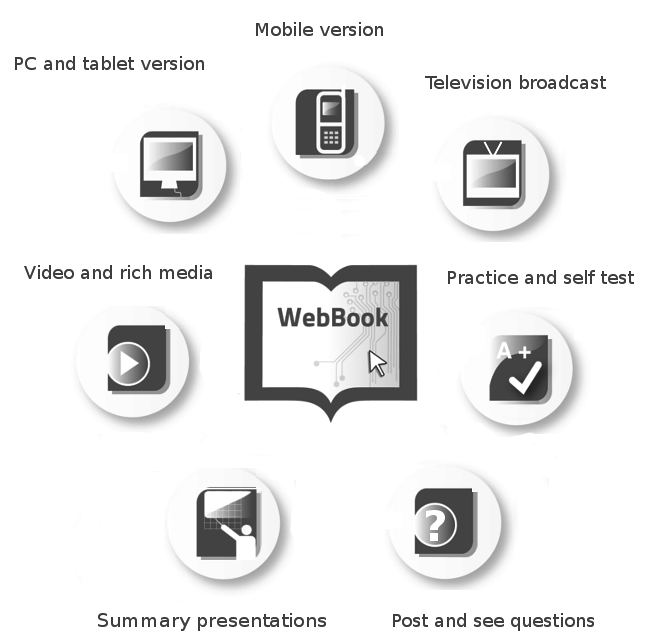
\includegraphics[width=0.70\textwidth]{title_images/morethantextbook.png}
\end{center}

\par
{\Large
\textbf{\textit{Everything Science}} is nie net ‘n Wetenskap handboek nie. Daar is meer in as net die gewone inhoud wat jy van ‘n skoolhandboek verwag. Om mee te begin kan jy die boek aflaai of aanlyn lees op jou selfoon, rekenaar of iPad. Dit is daarom gerieflik beskikbaar waar ook al jy is.\par


Ons weet dat dit partykeer moeilik is om iets in woorde te verduidelik, daarom is daar lesse en verduidelikings in video-formaat by elke hoofstuk sodat die idees en konsepte vir jou realiteit kan word. Die aanbieding aan die einde van elke hoofstuk bied ‘n oorsig oor al die inhoud wat jy geleer het, en die kern konsepte is vir jou uitgelig sodat jy die maklik kan hersien.\par


Al die oefeninge in die boek het ‘n skakel na ‘n diens wat vir jou nog oefeninge gee, die oplossings gee of jou toelaat om jou vaardigheid te toets – op ‘n selfoon of ‘n rekenaar.\par


Ons wil weet wat jy dink, waaroor jy wonder, en waarmee jy sukkel terwyl jy deur die boek werk en die oefeninge probeer doen. Ons het dit daarom moontlik gemaak dat jy jou werk, met jou selfoon of rekenaar, digitaal kan “aansteek” op ‘n bladsy en dan ook te kan sien watter vrae en antwoorde ander lesers “aangesteek” het.\par


% Mindset Learn gebruik hierdie boek in hul nuwe televisiereeks waar ervare onderwysers deur die boek werk, konsepte verduidelik en oefeninge uit die boek uitwerk.
}




% mobile or PC
\newpage
\thispagestyle{empty}

{\normalfont\sffamily\fontsize{22}\normalfont\itshape Everything Science op jou selfoon of rekenaar} \par

{\Large
Jy het altyd toegang  tot die handboek, of jy by die huis,die skool of op ‘n trein is. Blaai deur na die aanlyn weergawe van Everything Science op jou selfoon, “tablet” of rekenaar. As jy dit wil lees terwyl jy van lyn af is, kan jy dit as ‘n PDF-leêr of in e-boek formaat aflaai.\par


Om te lees of dit aflaai, gaan na \ textbf {www.everythingscience.co.za} op jou selfoon of rekenaar.} \vspace*{2cm}


\begin{center}
\begin{minipage}{0.4\textwidth}
\centering
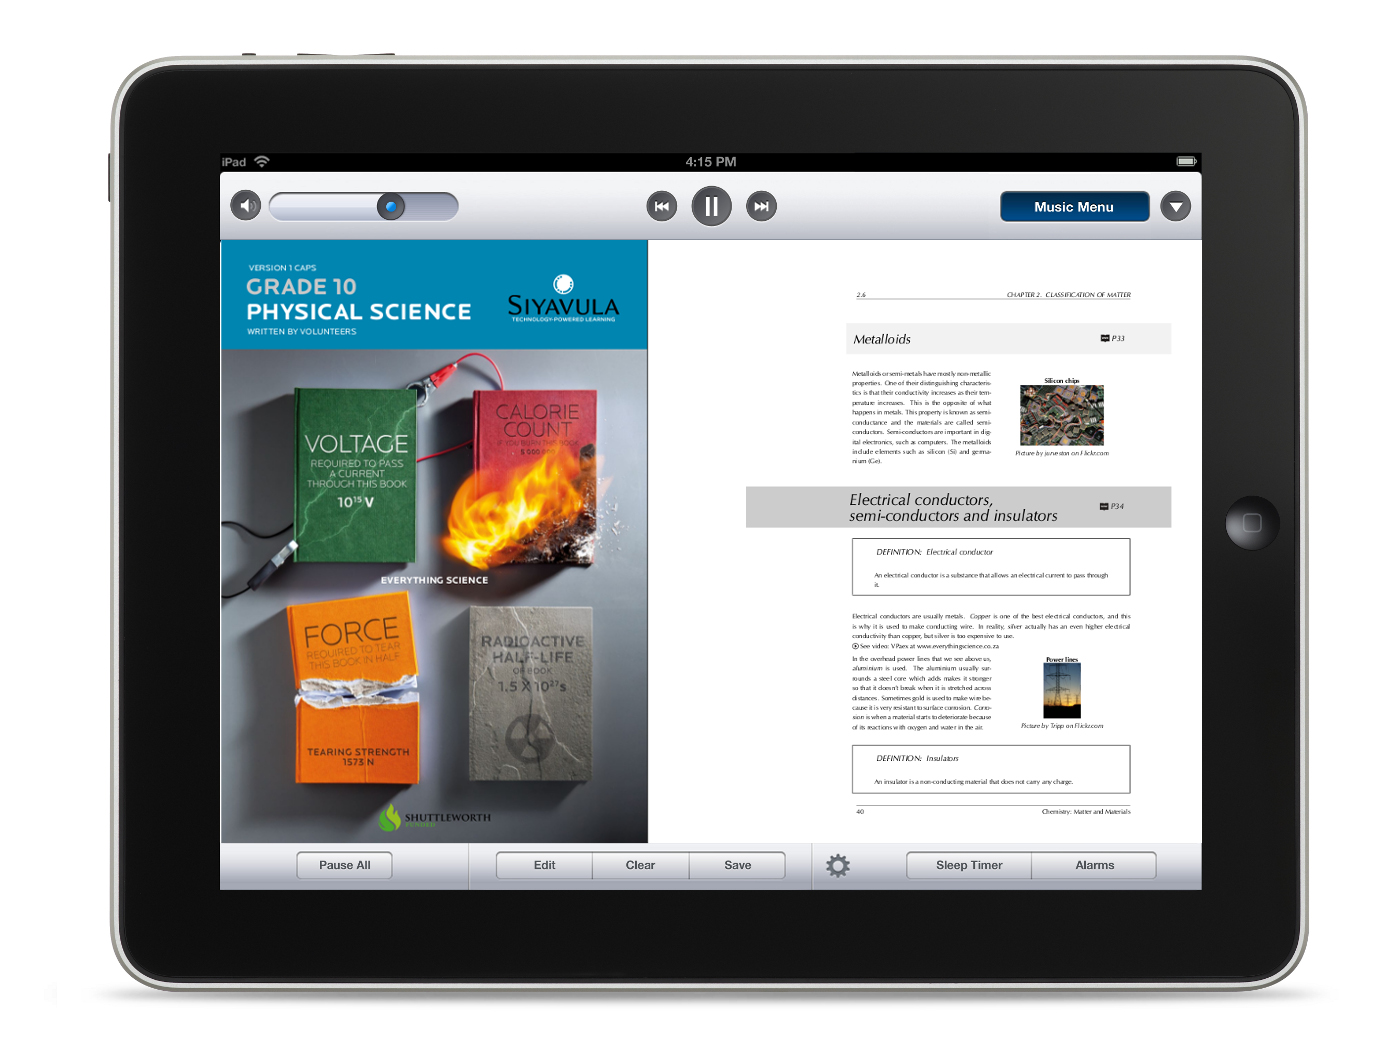
\includegraphics[width=0.8\textwidth]{title_images/ipad.jpg}
\end{minipage}
\begin{minipage}{0.4\textwidth}
\centering
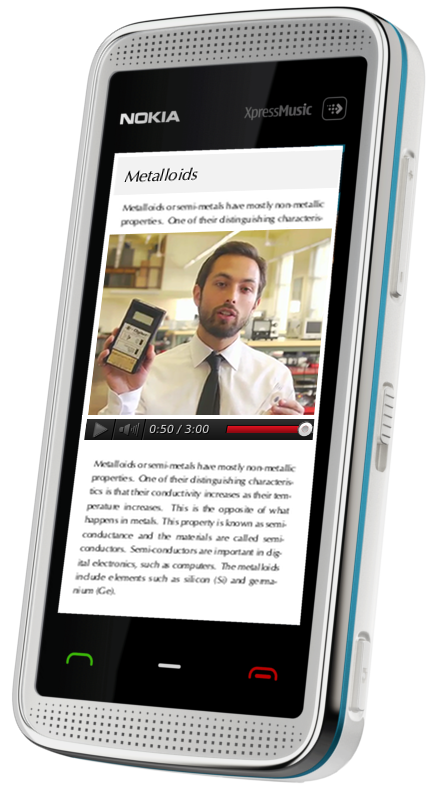
\includegraphics[width=0.4\textwidth]{title_images/phone.png}
\end{minipage}
\end{center}

\vspace*{2cm}


{\normalfont\sffamily\fontsize{22}\normalfont\itshape Hoe om die ikons en kortkodes te gebruik} \par

{\Large
Die ikons in die boek help jou om te sien waar videos, aanbiedinge, oefeninge en ander hulp voorkom. Die short-codes langs die ikons laat jou toe om direk na die aanlyn-bron te blaai sonder om daarvoor te soek.\par


\begin{tabular}{lcl}
\raisebox{-0.8em}{
\includegraphics[width=0.8cm]{../icons/www.pdf}} & (A123) & Gaan direk na 'n afdeling \\
\raisebox{-0.8em}{
\includegraphics[width=0.8cm]{../icons/video.pdf}} & (V123) & Video, simulasie of aanbieding \\
\raisebox{-0.8em}{
\includegraphics[width=0.8cm]{../icons/aplus.pdf}} & (P123) & Oefen en toets jou vaardighede \\
\raisebox{-0.8em}{
\includegraphics[width=0.8cm]{../icons/help.pdf}} & (Q123) & Vra vir hulp of vind 'n antwoord \\
\end{tabular}
\par
\vspace*{1cm}

Om die videos aanlyn te sien, oefeninge te doen of ‘n vraag op te sit, gaan na die \textit{Everything Science} webblad by \textbf{www.everythingscience.co.za} van jou selfoon of rekenaar en voer die kortkode in die soek-blokkie in.
}




% video lessons
\newpage
\thispagestyle{empty}

{\normalfont\sffamily\fontsize{22}\normalfont\itshape Video-lesse} \par

{\Large

Soek die video ikons in die boek. Hierdie ikons neem jou na video-lesse wat deur Mindset Learn gemaak is, wat sal help om die idees en konsepte vir jou lewendig te maak. Jy kan ekstra insigte, volledige verduidelikings en uitgewerkte voorbeelde hier sien. Die konsep word prakties voorgestel en jy kan luister hoe regte mense wiskunde en wetenskap in hul werk gebruik. \par

\begin{center}
Sien video verduideliking \raisebox{-0.6em}{
\includegraphics[width=0.7cm]{../icons/video.pdf}} (Video: V123)\\
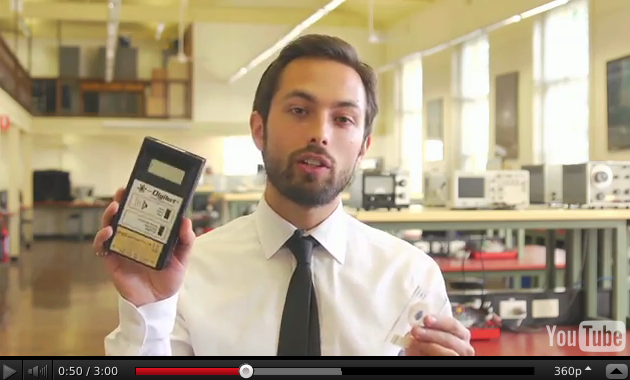
\includegraphics[width=0.5\textwidth]{title_images/veritasiumvideo.png}
\end{center}\par

}
\vspace{0.5cm}
{\normalfont\sffamily\fontsize{22}\normalfont\itshape Video exercises} \par

{\Large

As daar oefeninge in die boek is, sal jy die ikons en short codes vir video-oplossings, oefeninge en hulp sien. Hierdie short-codes vat jou na die video-oplossings van sommige oefeninge sodat jy stap-vir-stap kan sien hoe om die probleem op te los. \par

\begin{center}
Sien video oefening \raisebox{-0.6em}{
\includegraphics[width=0.7cm]{../icons/video.pdf}} (Video: V123) \\
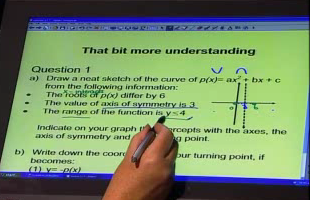
\includegraphics[width=0.5\textwidth]{title_images/mindsetexercise.png}
\end{center}
\par
Jy kan toegang tot die videos kry deur:
\begin{itemize}
    \item hulle aanlyn op jou selfoon of rekenaar te kyk
    \item die videos af te laai sodat jy die van lyn af op jou selfoon of rekenaar kan kyk
    \item ‘n DVD te bestel wat jy op jou TV of rekenaar kan speel
    \item dit van lyn af af te laai met Bluetooth of Wi-Fi van sekere afsetpunte
\end{itemize}
}


% practise and test your skills
\newpage
\thispagestyle{empty}
{\Large

Om nog videos te sien, videos af te laai of vir meer inligting, besoek die Everything Science webblad van jou selfoon of rekenaar af \underline{www.everythingscience.co.za}  \par
\vspace*{1cm}
{\normalfont\sffamily\fontsize{22}\normalfont\itshape Oefen en toets jou vaardigheid} \par


Een van die beste maniere om vir toetse of eksamens voor te berei, is om te oefen om dieselfde soort vrae te antwoord as waarmee jy getoets gaan word. By elke stel oefeninge is daar ‘n oefen ikon en ‘n short-code. Hierdie aanlyn-oefeninge, wat jy van jou \textbf{selfoon} of \textbf{rekenaar} af lan laai, hou rekord van jou prestasie en vordering, gee vir jou terugvoer oor watter areas jy mee sukkel en maak voorstelle oor na watter afdelings of videos jy moet gaan kyk.

\begin{center}
Sien meer oefeninge \raisebox{-0.6em}{
\includegraphics[width=0.7cm]{../icons/aplus.pdf}} (QM123) \\
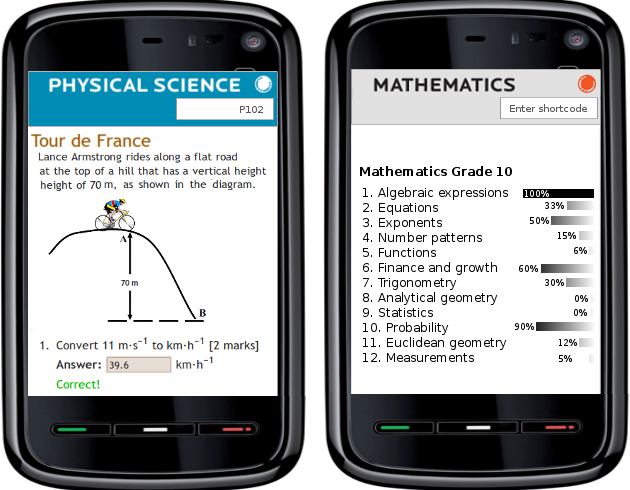
\includegraphics[width=0.65\textwidth]{title_images/practicephones.png}
\end{center}
\par



Om te oefen en jou vaardigheid te toets:\par

Gaan na \underline{www.everythingscience.co.za} van jou selfoon of rekenaar af en voer die kortkode in.\par

\vspace*{1cm}


%{\normalfont\sffamily\fontsize{22}\normalfont\itshape Television broadcasts} \par
%This book is the same one used by \textbf{Mindset Learn} in their television broadcast where experienced
%educators explain the key concepts, perform live experiments and work out exercises from the book.
%\textbf{Mindset Learn} broadcasts a full 28 hours of curriculum support each week of term. \par
%
%
%Maths can be seen on Mondays and Science on Tuesdays. There is also Life Sciences on Wednesdays
%and Maths Literacy on Thursdays. Revision of the week's work is done on Saturdays for Grade 12 and on
%Sundays for Grades 10 and 11.
%

}

\newpage
\thispagestyle{empty}

{\normalfont\sffamily\fontsize{22}\normalfont\itshape Vra vrae en vind antwoorde} \par

{\Large

Het jy al ooit 'n vraag oor' n spesifieke feit, formule of 'n oefening in jou handboek en wens jy kon net iemand vra om? Sekerlik moes iemand anders in die land gehad het dieselfde vraag op dieselfde plek in die handboek.\par 

Ons nooi u die handboek op jou selfoon of rekenaar oop te maak en om jou vraag te pen op daardie presiese plek in die handboek vir die gebruik van die kortkode. Jy sal in staat wees om te sien of dit al voorheen gevra en wat is die antwoord op daardie vraag.\par

Die kortkodes op artikel opskrifte help jy na dele in die boek vrae te vra en te kyk vir daardie afdeling. Die kort kodes vir die oefeninge kan jy kyk na die vrae en antwoorde met betrekking tot daardie spesifieke oefeninge.\par

\begin{tabular}{lcl}
\raisebox{-0.8em}{
\includegraphics[width=0.8cm]{../icons/www.pdf}} & (A123) & Besoek hierdie afdeling om vrae te kyk of te pos\\
\raisebox{-0.8em}{
\includegraphics[width=0.8cm]{../icons/help.pdf}} & (Q123) & Vrae of help met 'n spesifieke vraag  \\
\end{tabular}



\begin{figure}[h]
\centering
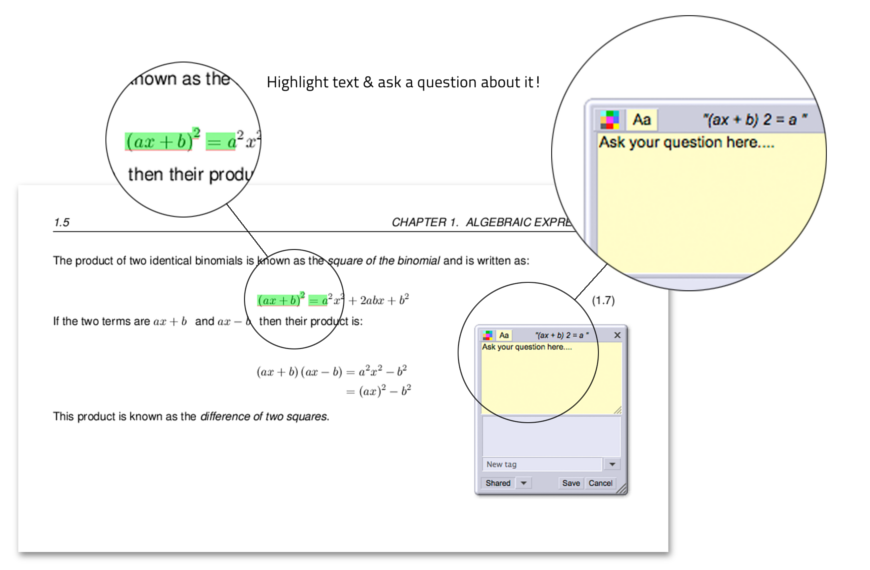
\includegraphics[width=\textwidth]{title_images/questions.png}
\end{figure}


}
%

%
%% practise and test your skills
%\newpage
%\thispagestyle{empty}
%{\Large
%
%\begin{table*}[h]
%\large
%\begin{tabular}{lll}
%\textbf{Maths and Science Broadcasts}&&\\
%Grade 10  Maths & Mondays at 4pm & Every second Sunday at 1pm\\
%Grade 11  Maths & Mondays at 5pm & Every second Sunday at 9am\\
%Grade 12  Maths & Mondays at 6pm & Every Saturday at 9am\\
%Grade 10  Science & Tuesdays at 4pm & Every second Sunday at 1pm\\
%Grade 11  Science & Tuesdays at 5pm & Every second Sunday at 9am\\
%Grade 12  Science & Tuesdays at 6pm & Every Saturday at 11am\\
%\textbf{Other broadcasts} & & \\
%Grade 10  Life Science & Wednesdays at 4pm & Every second Sunday at 3pm\\
%Grade 11  Life Science & Wednesdays at 5pm & Every second Sunday at 9am\\
%Grade 12  Life Science & Wednesdays at 6pm & Every Saturday at 1pm\\
%Grade 10  Maths Literacy & Thursdays at 4pm & Every second Sunday at 3pm\\
%Grade 11  Maths Literacy & Thursdays at 5pm & Every second Sunday at 9am\\
%Grade 12  Maths Literacy & Thursdays at 6pm & Every Saturday at 3pm\\
%\end{tabular}
%\end{table*}
%
%
%\textbf{You can watch these live sessions on:}
%\begin{itemize}
%    \item Mindset free-to-air for schools (ask your school)
%    \item Channels 319 on DStv
%    \item Toptv on 319 on TopTV
%\end{itemize}


%}

% Put the margins back for the rest of the book

\newgeometry{lmargin=0.1\paperwidth, rmargin=0.25\paperwidth, tmargin=1in, bmargin=1in, twoside, centering, includehead,  marginparwidth=0.225\paperwidth}

\normalfont
